\section{Specific Requirements}

\subsection{External Interfaces}

\vfill
\begin{figure}[H]
  \centering
  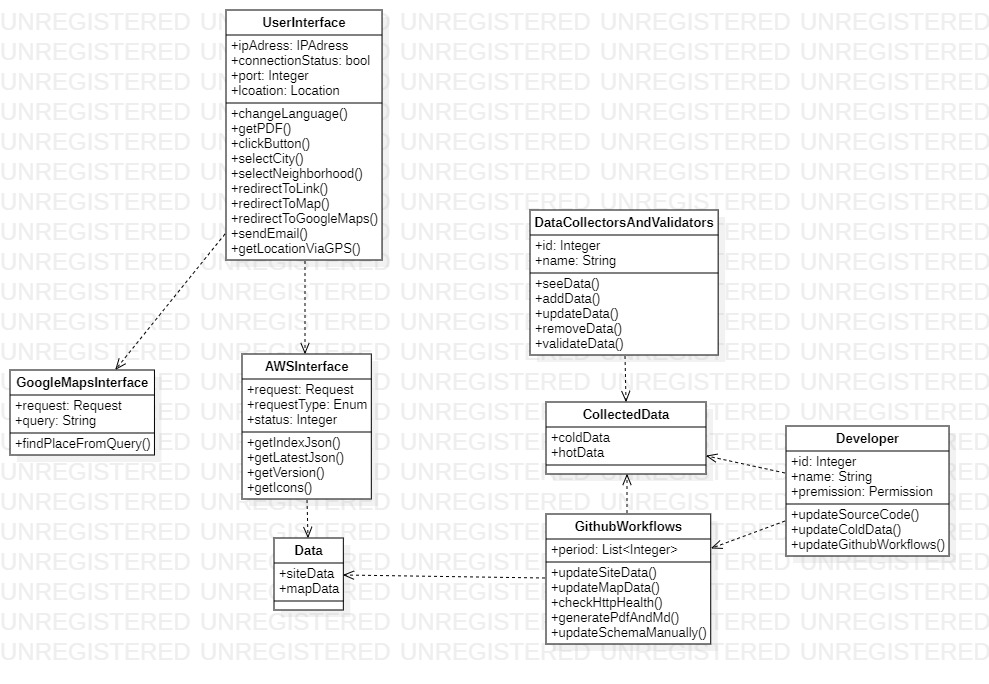
\includegraphics[width=\linewidth]{img/external-interfaces.jpg}
  \caption{External Interfaces}
\end{figure}
\vfill
\newpage

\subsection{Functions}

\vfill
\begin{figure}[H]
  \centering
  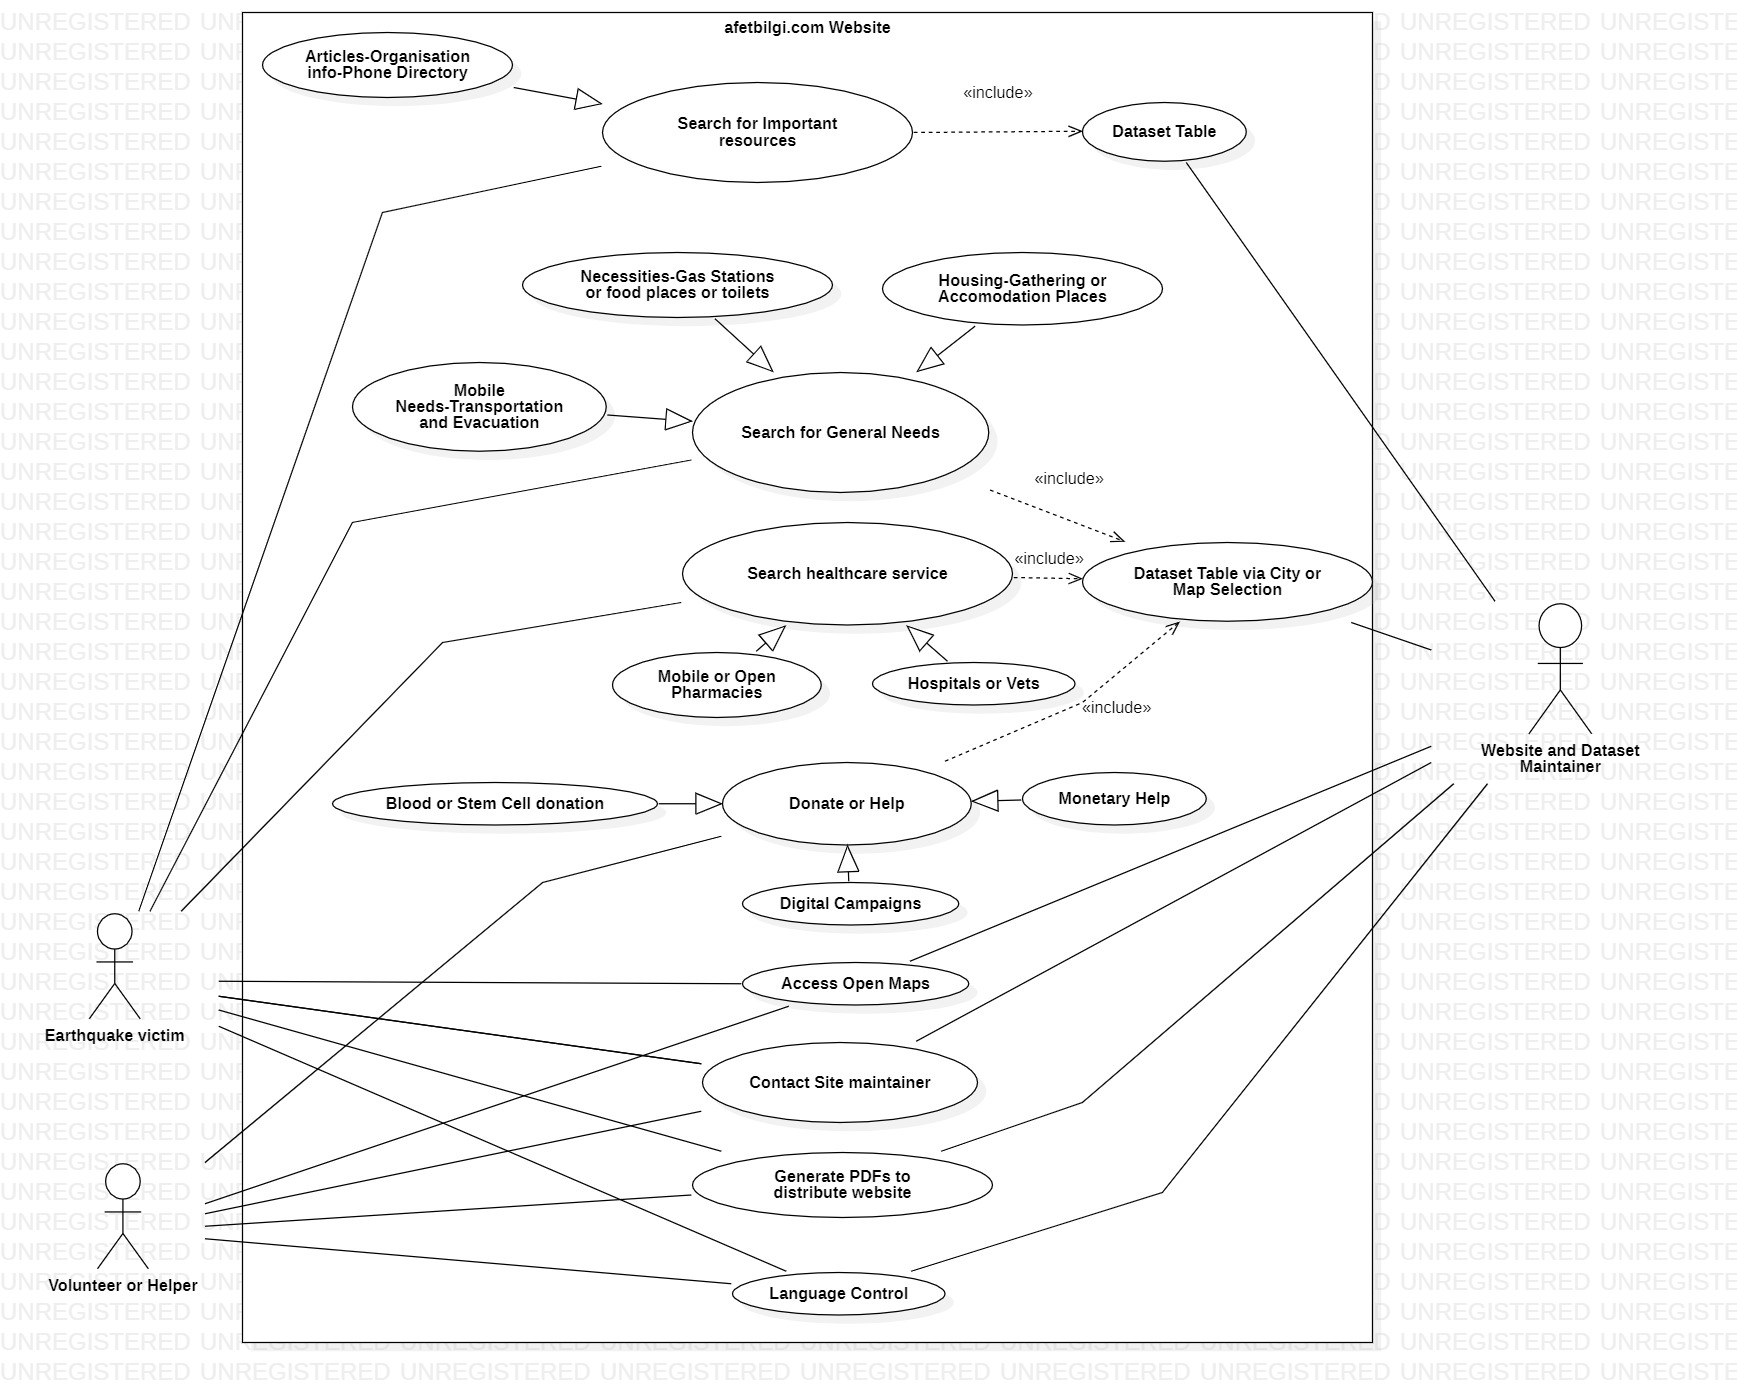
\includegraphics[width=\linewidth]{img/use-case-diagram.jpg}
  \caption{Use Case Diagram for \afetbilgi}
\end{figure}
\vfill
\newpage

% Search for important resources
\begin{table}[H]
  \centering
  \refstepcounter{useCaseID}
  \resizebox{\linewidth}{!}{%
    \begin{tabular}{|p{.3\linewidth}|p{.7\linewidth}|}
      \hline
      \textbf{Use Case ID} & \theuseCaseID \\
      \hline
      \textbf{Use-Case Name} & Search for important resources \\
      \hline
      \textbf{Actors} & Victims or volunteers and Website maintainers \\
      \hline
      \textbf{Description} & Whenever a site user wants to display a important resource, he or she can view verified and updated resources such as crucial phone numbers and websites, which he or she can acquire necessary information. \\
      \hline
      \textbf{Data} & Verified and updated table of important resources such as crucial phones and website, and articles. \\
      \hline
      \textbf{Preconditions} & The directory must be updated and verified regularly for potential update on the related information. \\
      \hline
      \textbf{Stimulus} & User clicks on the relevant important resource listed as bold text buttons under the ``\texttt{Important Resources}'' category on the website. \\
      \hline
      \textbf{Basic Flow} & 
        \begin{minipage}[H]{\linewidth} 
          \begin{enumerate}[label=\textbf{Step \arabic*:},leftmargin=1.5\leftmargin]
            \item User clicks on ``\texttt{Crucial Phone Number}''
            \item User displays the crucial phone numbers and related information to that phone number
          \end{enumerate}
        \end{minipage} \\
      \hline
      \textbf{Alternative Flow \#1} & 
        \begin{minipage}[H]{\linewidth} 
            \begin{enumerate}[label=\textbf{Step \arabic*:},leftmargin=1.5\leftmargin]
              \item User clicks on ``\texttt{Important Web Sites}''
              \item User displays the websites with their name and external links
              \item User clicks any of the presented external third party links
              \item User redirected to verified third party website
          \end{enumerate}
        \end{minipage} \\
      \hline
      \textbf{Alternative Flow \#2} &
        \begin{minipage}[H]{\linewidth} 
          \begin{enumerate}[label=\textbf{Step \arabic*:},leftmargin=1.5\leftmargin]
            \item User clicks on ``\texttt{Useful Articles}''
            \item User displays the titles and authors of the articles with an external links
            \item User clicks any of the presented external third party links
            \item User redirected to verified third party website
          \end{enumerate}
        \end{minipage} \\
      \hline
      \textbf{Exception Flow} & - \\
      \hline
      \textbf{Post Conditions} & User is redirected to a verified external website out of the \afetbilgi\ domain \\
      \hline
    \end{tabular}
  }
  \caption{Use Case - Search for important resources}
\end{table}

% Search for general needs 1
\begin{table}[H]
  \centering
  \refstepcounter{useCaseID}
  \resizebox{\linewidth}{!}{%
    \begin{tabular}{|p{.3\linewidth}|p{.7\linewidth}|}
      \hline
      \textbf{Use Case ID} & \theuseCaseID \\
      \hline
      \textbf{Use-Case Name} & Search for general needs $|$ Housing \\
      \hline
      \textbf{Actors} & Victims or volunteers and Website maintainers \\
      \hline
      \textbf{Description} & Whenever a site user wants to display elements related to housing in general needs, he or she can view verified and updated related lists, which he or she can acquire necessary information. \\
      \hline
      \textbf{Data} & Verified and updated table of general needs such as gathering and accommodation places. \\
      \hline
      \textbf{Preconditions} & The directory must be updated and verified regularly for potential update on the information. \\
      \hline
      \textbf{Stimulus} & User clicks on the relevant general need listed as bold text buttons under the ``\texttt{General Needs}'' category on the website. \\
      \hline
      \textbf{Basic Flow} & 
        \begin{minipage}[H]{\linewidth} 
          \begin{enumerate}[label=\textbf{Step \arabic*:},leftmargin=1.5\leftmargin]
            \item User clicks on ``\texttt{Safe Gathering Places}''
            \item User selects city where he or she want to get related information
            \item User displays the list of safe gathering areas in selected city with map link to the address and source of the information
            \item User clicks map or source link
            \item User is redirected to google maps or the source
          \end{enumerate}
        \end{minipage} \\
      \hline
      \textbf{Alternative Flow \#1} & 
        \begin{minipage}[H]{\linewidth} 
          \begin{enumerate}[label=\textbf{Step \arabic*:},leftmargin=1.5\leftmargin]
            \item User clicks on ``\texttt{Temporary Accommodation Places}''
            \item User displays list of places from national temporary accommodations or selects city where he or she want to get related information
            \item User displays the list of temporary accommodation places in selected city with location link and details
            \item User clicks location link
            \item User is redirected to google maps
          \end{enumerate}
        \end{minipage} \\
      \hline
      \textbf{Alternative Flow \#2} & - \\
      \hline
      \textbf{Exception Flow} & - \\
      \hline
      \textbf{Post Conditions} & User is redirected to a verified external website out of the \afetbilgi\ domain \\
      \hline
    \end{tabular}
  }
  \caption{Use Case - Search for general needs $|$ Housing}
\end{table}

% Search for general needs 2
\begin{table}[H]
  \centering
  \refstepcounter{useCaseID}
  \resizebox{\linewidth}{!}{%
    \begin{tabular}{|p{.3\linewidth}|p{.7\linewidth}|}
      \hline
      \textbf{Use Case ID} & \theuseCaseID \\
      \hline
      \textbf{Use-Case Name} & Search for general needs $|$ Necessities \\
      \hline
      \textbf{Actors} & Victims or volunteers and Website maintainers \\
      \hline
      \textbf{Description} & Whenever a site user wants to display elements related to necessities in general needs, he or she can view verified and updated related lists, which he or she can acquire necessary information. \\
      \hline
      \textbf{Data} & Verified and updated table of general needs such as gas stations, food places or toilets. \\
      \hline
      \textbf{Preconditions} & The directory must be updated and verified regularly for potential update on the information. \\
      \hline
      \textbf{Stimulus} & User clicks on the relevant general need listed as bold text buttons under the ``\texttt{General Needs}'' category on the website. \\
      \hline
      \textbf{Basic Flow} & 
        \begin{minipage}[H]{\linewidth} 
          \begin{enumerate}[label=\textbf{Step \arabic*:},leftmargin=1.5\leftmargin]
            \setlength{\itemsep}{1pt}
            \item User clicks on ``\texttt{Gas Stations}''
            \item User selects city where he or she want to get related information
            \item User selects the county where he or she want to get related information
            \item User displays the list of gas stations in selected area with location link and contact information
            \item User clicks location or contact link
            \item User is redirected to google maps or phone app
          \end{enumerate}
        \end{minipage} \\
      \hline
      \textbf{Alternative Flow \#1} & 
        \begin{minipage}[H]{\linewidth} 
          \begin{enumerate}[label=\textbf{Step \arabic*:},leftmargin=1.5\leftmargin]
            \setlength{\itemsep}{1pt}
            \item User clicks on ``\texttt{Food Distribution Center}''
            \item User displays list of places from national temporary accommodations or selects city where he or she want to get related information
            \item User selects county
            \item User displays the list of food distribution locations in selected city with location link and details
            \item User clicks location link
            \item User is redirected to google maps
          \end{enumerate}
        \end{minipage} \\
      \hline
      \textbf{Alternative Flow \#2} &
        \begin{minipage}[H]{\linewidth} 
          \begin{enumerate}[label=\textbf{Step \arabic*:},leftmargin=1.5\leftmargin]
            \setlength{\itemsep}{1pt}
            \item User clicks on ``\texttt{Mobile Toilets Articles}''
            \item User redirected to verified source
          \end{enumerate}
        \end{minipage} \\
      \hline
      \textbf{Exception Flow} & - \\
      \hline
      \textbf{Post Conditions} & User is redirected to a verified external website out of the \afetbilgi\ domain \\
      \hline
    \end{tabular}
  }
  \caption{Use Case - Search for general needs $|$ Necessities}
\end{table}

% Search for general needs 3
\begin{table}[H]
  \centering
  \refstepcounter{useCaseID}
  \resizebox{\linewidth}{!}{%
    \begin{tabular}{|p{.3\linewidth}|p{.7\linewidth}|}
      \hline
      \textbf{Use Case ID} & \theuseCaseID \\
      \hline
      \textbf{Use-Case Name} & Search for general needs $|$ Mobile needs \\
      \hline
      \textbf{Actors} & Victims or volunteers and Website maintainers \\
      \hline
      \textbf{Description} & Whenever a site user wants to display elements related to mobile elements in general needs, he or she can view verified and updated related lists, which he or she can acquire necessary information. \\
      \hline
      \textbf{Data} & Verified and updated table of general needs such as transportation and evacuation. \\
      \hline
      \textbf{Preconditions} & The directory must be updated and verified regularly for potential update on the information. \\
      \hline
      \textbf{Stimulus} & User clicks on the relevant general need listed as bold text buttons under the ``\texttt{General Needs}'' category on the website. \\
      \hline
      \textbf{Basic Flow} & 
        \begin{minipage}[H]{\linewidth} 
            \begin{enumerate}[label=\textbf{Step \arabic*:},leftmargin=1.5\leftmargin]
              \item User clicks on ``\texttt{Transportation Aid}''
              \item User displays the list of transportation aids with name, details, validity and source of the information
              \item User clicks source link
              \item User is redirected to external third party website
            \end{enumerate}
        \end{minipage} \\
      \hline
      \textbf{Alternative Flow \#1} & 
        \begin{minipage}[H]{\linewidth} 
          \begin{enumerate}[label=\textbf{Step \arabic*:},leftmargin=1.5\leftmargin]
            \item User clicks on ``\texttt{evacuation Points}''
            \item User selects city where he or she want to get related information
            \item User displays the list of evacuation points with address, map link and contact information
            \item User clicks map or contact link
            \item User is redirected to google maps or phone app
          \end{enumerate}
        \end{minipage} \\
      \hline
      \textbf{Alternative Flow \#2} & - \\
      \hline
      \textbf{Exception Flow} & - \\
      \hline
      \textbf{Post Conditions} & User is redirected to a verified external website out of the \afetbilgi\ domain \\
      \hline
    \end{tabular}
  }
  \caption{Use Case - Search for general needs $|$ Mobile needs}
\end{table}

% Search for healthcare 1
\begin{table}[H]
  \centering
  \refstepcounter{useCaseID}
  \resizebox{\linewidth}{!}{%
    \begin{tabular}{|p{.3\linewidth}|p{.7\linewidth}|}
      \hline
      \textbf{Use Case ID} & \theuseCaseID \\
      \hline
      \textbf{Use-Case Name} & Search for healthcare $|$ Pharmacy \\
      \hline
      \textbf{Actors} & Victims or volunteers and Website maintainers \\
      \hline
      \textbf{Description} & Whenever a site user wants to display a pharmacy element in health services, he or she can view verified and updated related lists, which he or she can acquire necessary information. \\
      \hline
      \textbf{Data} & Verified and updated table of health services such as container and open pharmacies. \\
      \hline
      \textbf{Preconditions} & The directory must be updated and verified regularly for potential update on the information. \\
      \hline
      \textbf{Stimulus} & User clicks on the relevant health service listed as bold text buttons under the ``\texttt{Health Services}'' category on the website. \\
      \hline
      \textbf{Basic Flow} & 
        \begin{minipage}[H]{\linewidth} 
          \begin{enumerate}[label=\textbf{Step \arabic*:},leftmargin=1.5\leftmargin]
            \item User clicks on ``\texttt{Container Pharmacies}''
            \item User displays the list of container pharmacies with city, district and location of the information
            \item User clicks location link
            \item User is redirected to google maps
          \end{enumerate}
        \end{minipage} \\
      \hline
      \textbf{Alternative Flow \#1} & 
        \begin{minipage}[H]{\linewidth} 
          \begin{enumerate}[label=\textbf{Step \arabic*:},leftmargin=1.5\leftmargin]
            \item User clicks on ``\texttt{Open Pharmacies}''
            \item User selects city where he or she want to get related information
            \item User selects county where he or she want to get related information
            \item User displays the list of open pharmacies with name, address, map link and contact information
            \item User clicks location link or contact information
            \item User is redirected to google maps or phone app
          \end{enumerate}
        \end{minipage} \\
      \hline
      \textbf{Alternative Flow \#2} & - \\
      \hline
      \textbf{Exception Flow} & - \\
      \hline
      \textbf{Post Conditions} & User is redirected to a verified external website or app out of the \afetbilgi\ domain \\
      \hline
    \end{tabular}
  }
  \caption{Use Case - Search for healthcare $|$ Pharmacy}
\end{table}

% Search for healthcare 2
\begin{table}[H]
  \centering
  \refstepcounter{useCaseID}
  \resizebox{\linewidth}{!}{%
    \begin{tabular}{|p{.3\linewidth}|p{.7\linewidth}|}
      \hline
      \textbf{Use Case ID} & \theuseCaseID \\
      \hline
      \textbf{Use-Case Name} & Search for healthcare $|$ Hospitals and Vets \\
      \hline
      \textbf{Actors} & Victims or volunteers and Website maintainers \\
      \hline
      \textbf{Description} & Whenever a site user wants to display a hospital or vet element in health services, he or she can view verified and updated related lists, which he or she can acquire necessary information. \\
      \hline
      \textbf{Data} & Verified and updated table of health services such as active hospitals and veterinarians. \\
      \hline
      \textbf{Preconditions} & The directory must be updated and verified regularly for potential update on the information. \\
      \hline
      \textbf{Stimulus} & User clicks on the relevant health service listed as bold text buttons under the ``\texttt{Health Services}'' category on the website. \\
      \hline
      \textbf{Basic Flow} & 
        \begin{minipage}[H]{\linewidth} 
          \begin{enumerate}[label=\textbf{Step \arabic*:},leftmargin=1.5\leftmargin]
            \item User clicks on ``\texttt{Active Hospitals}''
            \item User selects city where he or she want to get related information
            \item User displays the list of active hospitals areas in selected city with map link to the address and source of the information
            \item User clicks location link
            \item User is redirected to google maps
          \end{enumerate}
        \end{minipage} \\
      \hline
      \textbf{Alternative Flow \#1} & 
        \begin{minipage}[H]{\linewidth} 
          \begin{enumerate}[label=\textbf{Step \arabic*:},leftmargin=1.5\leftmargin]
            \item User clicks on ``\texttt{Veterinarians}''
            \item User selects city where he or she want to get related information
            \item User displays the list of veterinarians in selected city with name, map link to the address and contact of the information
            \item User clicks map link or contact information
            \item User is redirected to google maps or phone app
          \end{enumerate}
        \end{minipage} \\
      \hline
      \textbf{Alternative Flow \#2} & - \\
      \hline
      \textbf{Exception Flow} & - \\
      \hline
      \textbf{Post Conditions} & User is redirected to a verified external website or app out of the \afetbilgi\ domain \\
      \hline
    \end{tabular}
  }
  \caption{Use Case - Search for healthcare $|$ Hospitals and Vets}
\end{table}

% Donate or Help 1
\begin{table}[H]
  \centering
  \refstepcounter{useCaseID}
  \resizebox{\linewidth}{!}{%
    \begin{tabular}{|p{.3\linewidth}|p{.7\linewidth}|}
      \hline
      \textbf{Use Case ID} & \theuseCaseID \\
      \hline
      \textbf{Use-Case Name} & Donate or Help $|$ Blood or Stem Cell Donation \\
      \hline
      \textbf{Actors} & Volunteers and Website maintainers \\
      \hline
      \textbf{Description} & Whenever a site user wants to donate blood or stem to earthquake victims, he or she can view verified and updated institutions and organisations, which he or she can donate to \\
      \hline
      \textbf{Data} & Verified and updated directory of external third party links of welfare and governmental organisations \\
      \hline
      \textbf{Preconditions} & The directory must be updated and verified regularly given the potential monetary usage of the links in the future by the users \\
      \hline
      \textbf{Stimulus} & User clicks on the relevant donation/help methods listed as bold text buttons in the ``\texttt{To Help}'' category on the website \\
      \hline
      \textbf{Basic Flow} & 
        \begin{minipage}[H]{\linewidth} 
          \begin{enumerate}[label=\textbf{Step \arabic*:},leftmargin=1.5\leftmargin]
            \item User clicks on ``\texttt{Kizilay Blood Donation Places}''
            \item User automatically redirected to primary verified third party site of governmental organisation accepting blood donations
          \end{enumerate}
        \end{minipage} \\
      \hline
      \textbf{Alternative Flow \#1} & 
        \begin{minipage}[H]{\linewidth} 
          \begin{enumerate}[label=\textbf{Step \arabic*:},leftmargin=1.5\leftmargin]
            \item User clicks on ``\texttt{Stem Cell Donation Points}''
            \item User displays the list of stem cell donation points with region, map link to the address and contact of the item
            \item User clicks map link or contact
            \item User is redirected to google map or phone app
          \end{enumerate}
        \end{minipage} \\
      \hline
      \textbf{Alternative Flow \#2} & - \\
      \hline
      \textbf{Exception Flow} & - \\
      \hline
      \textbf{Post Conditions} & User is redirected to a verified external website out of the \afetbilgi\ domain \\
      \hline
    \end{tabular}
  }
  \caption{Use Case - Donate or Help $|$ Blood or Stem Cell Donation}
\end{table}

% Donate or Help 2
\begin{table}[H]
  \centering
  \refstepcounter{useCaseID}
  \resizebox{\linewidth}{!}{%
    \begin{tabular}{|p{.3\linewidth}|p{.7\linewidth}|}
      \hline
      \textbf{Use Case ID} & \theuseCaseID \\
      \hline
      \textbf{Use-Case Name} & Donate or Help $|$ Digital Campaigns and Other Donation \\
      \hline
      \textbf{Actors} & Volunteers and Website maintainers \\
      \hline
      \textbf{Description} & Whenever a site user wants to donate to digital campaigns to help earthquake victims, he or she can view verified and updated institutions and organisations, which he or she can donate to \\
      \hline
      \textbf{Data} & Verified and updated directory of external third party links of welfare and governmental organisations \\
      \hline
      \textbf{Preconditions} & The directory must be updated and verified regularly given the potential monetary usage of the links in the future by the users \\
      \hline
      \textbf{Stimulus} & User clicks on the relevant donation/help methods listed as bold text buttons in the ``\texttt{To Help}'' category on the website \\
      \hline
      \textbf{Basic Flow} & 
        \begin{minipage}[H]{\linewidth} 
          \begin{enumerate}[label=\textbf{Step \arabic*:},leftmargin=1.5\leftmargin]
            \item User clicks on ``\texttt{Digital solidarity campaigns}''
            \item User selects any of the presented external-3rd party links(presented in a directory)
            \item User redirected to verified 3rd party website
          \end{enumerate}
        \end{minipage} \\
      \hline
      \textbf{Alternative Flow \#1} & 
        \begin{minipage}[H]{\linewidth} 
          \begin{enumerate}[label=\textbf{Step \arabic*:},leftmargin=1.5\leftmargin]
            \item User clicks on ``\texttt{Other donation}''
            \item User selects relevant city
            \item User selects verified helper links of individuals/smaller organisations along with their contact details
            \item User clicks on any link and escorted out to a 3rd party site
          \end{enumerate}
        \end{minipage} \\
      \hline
      \textbf{Alternative Flow \#2} & - \\
      \hline
      \textbf{Exception Flow} & - \\
      \hline
      \textbf{Post Conditions} & User is redirected to a verified external website out of the \afetbilgi\ domain \\
      \hline
    \end{tabular}
  }
  \caption{Use Case - Donate or Help $|$ Digital Campaigns and Other Donation}
\end{table}

% Donate or Help 3
\begin{table}[H]
  \centering
  \refstepcounter{useCaseID}
  \resizebox{\linewidth}{!}{%
    \begin{tabular}{|p{.3\linewidth}|p{.7\linewidth}|}
      \hline
      \textbf{Use Case ID} & \theuseCaseID \\
      \hline
      \textbf{Use-Case Name} & Donate or Help $|$ Monetary Help \\
      \hline
      \textbf{Actors} & Volunteers and Website maintainers \\
      \hline
      \textbf{Description} & Whenever a site user wants to donate or help earthquake victims, he or she can view verified and updated institutions and organisations, which he or she can donate to \\
      \hline
      \textbf{Data} & Verified and updated directory of external 3rd party links of welfare and governmental organisations \\
      \hline
      \textbf{Preconditions} & The directory must be updated and verified regularly given the potential monetary usage of the links in the future by the users \\
      \hline
      \textbf{Stimulus} & User clicks on the relevant donation/help methods listed as bold text buttons in the ``\texttt{To Help}'' category on the website \\
      \hline
      \textbf{Basic Flow} & 
        \begin{minipage}[H]{\linewidth} 
          \begin{enumerate}[label=\textbf{Step \arabic*:},leftmargin=1.5\leftmargin]
            \item User clicks on ``\texttt{Monetary Dotation Link}''
            \item User displays a list of institutions and organizations with map link to address location and contact link
            \item User clicks map link or contact
            \item User is redirected to google map or phone app
          \end{enumerate}
        \end{minipage} \\
      \hline
      \textbf{Alternative Flow \#1} & - \\
      \hline
      \textbf{Alternative Flow \#2} & - \\
      \hline
      \textbf{Exception Flow} & - \\
      \hline
      \textbf{Post Conditions} & User is redirected to a verified external website out of the \afetbilgi\ domain \\
      \hline
    \end{tabular}
  }
  \caption{Donate or Help $|$ Monetary Help}
\end{table}

% Activity Diagram - Donate or Help
\begin{figure}[H]
  \centering
  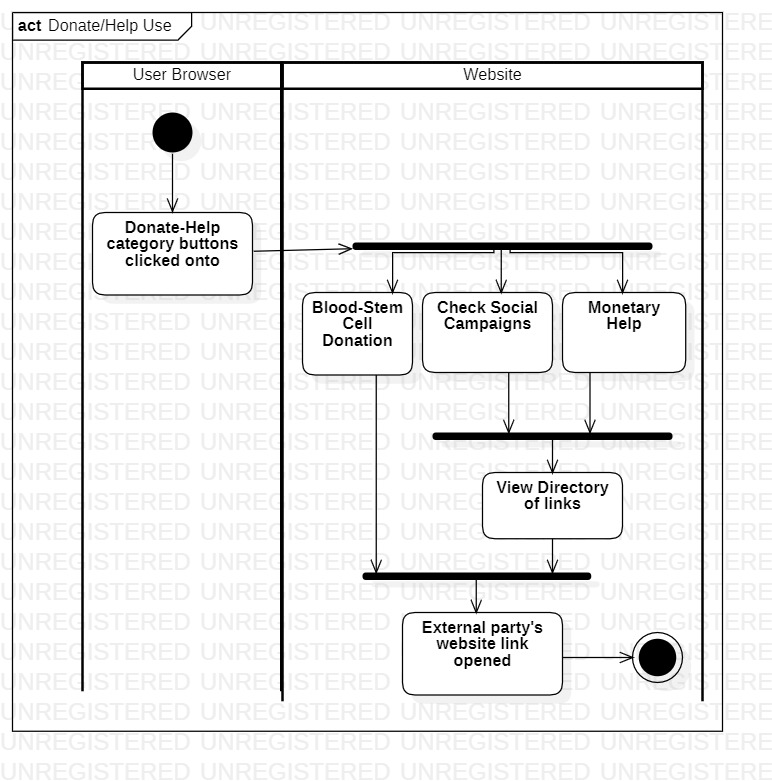
\includegraphics[width=\linewidth]{img/activity-diagram-donate-or-help.jpg}
  \caption{Activity Diagram - Donate or Help}
\end{figure}

\vspace*{\fill}
\newpage

% Access open maps
\begin{table}[H]
  \centering
  \refstepcounter{useCaseID}
  \resizebox{\linewidth}{!}{%
    \begin{tabular}{|p{.3\linewidth}|p{.7\linewidth}|}
      \hline
      \textbf{Use Case ID} & \theuseCaseID \\
      \hline
      \textbf{Use-Case Name} & Access open maps \\
      \hline
      \textbf{Actors} & Volunteers or Victims, Website maintainers \\
      \hline
      \textbf{Description} & Users can view current location with respect to places in need of help and use interactive map view to track down relevant places offering help (verified by site maintainers) via GPS location \\
      \hline
      \textbf{Data} & Interactive Map View with relevant place descriptions to navigate on \\
      \hline
      \textbf{Preconditions} & Places ought to be verified, properly categorised and color coded for easy understanding by site user \\
      \hline
      \textbf{Stimulus} & User drags mouse around on map view involving GPS after clicking on the map button anywhere on screen or calling \href{https://maps.afetbilgi.com}{\texttt{maps.afetbilgi.com}} directly in the browser \\
      \hline
      \textbf{Basic Flow} & 
          \begin{minipage}[H]{\linewidth} 
              \begin{enumerate}[label=\textbf{Step \arabic*:},leftmargin=1.5\leftmargin]
                  \item User is shown his current location with respect to to rest of Turkey
                  \item Users can zoom in or out of Turkey's map and track themselves to needy areas as per color codes and categorisation
                  \item User can click on a tracked down helping house, restaurant, etc. and be greeted by a pop up box with description and relevant links to third party sites or Google Maps routes
                  \item User can click on the links and escorted out to 3rd party websites or Google Maps website
              \end{enumerate}
          \end{minipage} \\
      \hline
      \textbf{Alternative Flow \#1} & 
      \begin{minipage}[H]{\linewidth} 
              \begin{enumerate}[label=\textbf{Step \arabic*:},leftmargin=1.5\leftmargin]
                  \item User can select zoom in or out along with clicking on the camera icon
                  \item User can save map screenshot for later use or distribution
              \end{enumerate}
          \end{minipage} \\
      \hline
      \textbf{Alternative Flow \#2} & - \\
      \hline
      \textbf{Exception Flow} & - \\
      \hline
      \textbf{Post Conditions} & User ends up on verified external website outside of \afetbilgi\ domain \\
      \hline
    \end{tabular}
  }
  \caption{Use Case - Access open maps}
\end{table}

% State Diagram - Access open maps
\begin{figure}[H]
  \centering
  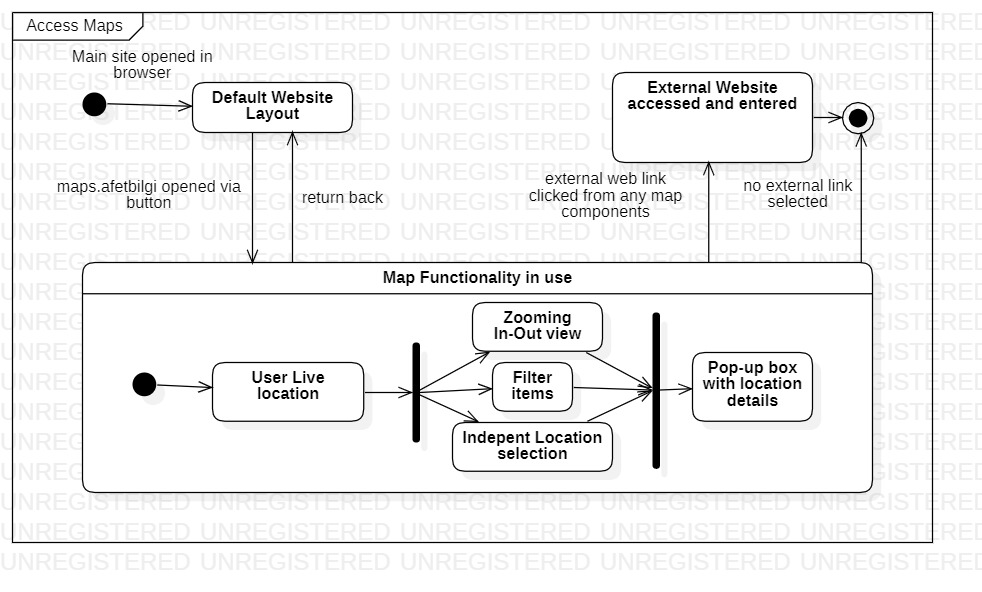
\includegraphics[width=\linewidth]{img/state-diagram-access-map.jpg}
  \caption{State Diagram - Acces Open Maps}
\end{figure}

\vfill
\newpage

% Generate PDFs to distribute website
\begin{table}[H]
  \centering
  \refstepcounter{useCaseID}
  \resizebox{\linewidth}{!}{%
    \begin{tabular}{|p{.3\linewidth}|p{.7\linewidth}|}
      \hline
      \textbf{Use Case ID} & \theuseCaseID \\
      \hline
      \textbf{Use-Case Name} & Generate PDFs to distribute website \\
      \hline
      \textbf{Actors} & Volunteers or victims \\
      \hline
      \textbf{Description} & Users can save filtered out website directories for later use given possible lack of electrical or network necessities in these earthquake stricken areas\\
      \hline
      \textbf{Data} & Separate downloadable PDF documents after selecting relevant cities \\
      \hline
      \textbf{Preconditions} & User is able to select entire cities with verified directory links and contact information  \\
      \hline
      \textbf{Stimulus} & User clicks on PDF icon button anywhere on the website \\
      \hline
      \textbf{Basic Flow} &
          \begin{minipage}[H]{\linewidth} 
              \begin{enumerate}[label=\textbf{Step \arabic*:},leftmargin=1.5\leftmargin]
                  \item User clicks on PDF icon anywhere on website
                  \item User selects city
                  \item Document is loaded and enabled for download by the user with the relevant city and categories highlighted on it
              \end{enumerate}
          \end{minipage} \\
      \hline
      \textbf{Alternative Flow \#1} & - \\
      \hline
      \textbf{Alternative Flow \#2} & - \\
      \hline
      \textbf{Exception Flow} & - \\
      \hline
      \textbf{Post Conditions} & Site user has received well formatted and legible generated PDF document with relevant hyperlinks and contact details of verified directories  \\
      \hline
    \end{tabular}
  }
  \caption{Use Case - Generate PDFs to distribute website}
\end{table}

% Sequence Diagram - Generate PDFs to distribute website
\begin{figure}[H]
  \centering
  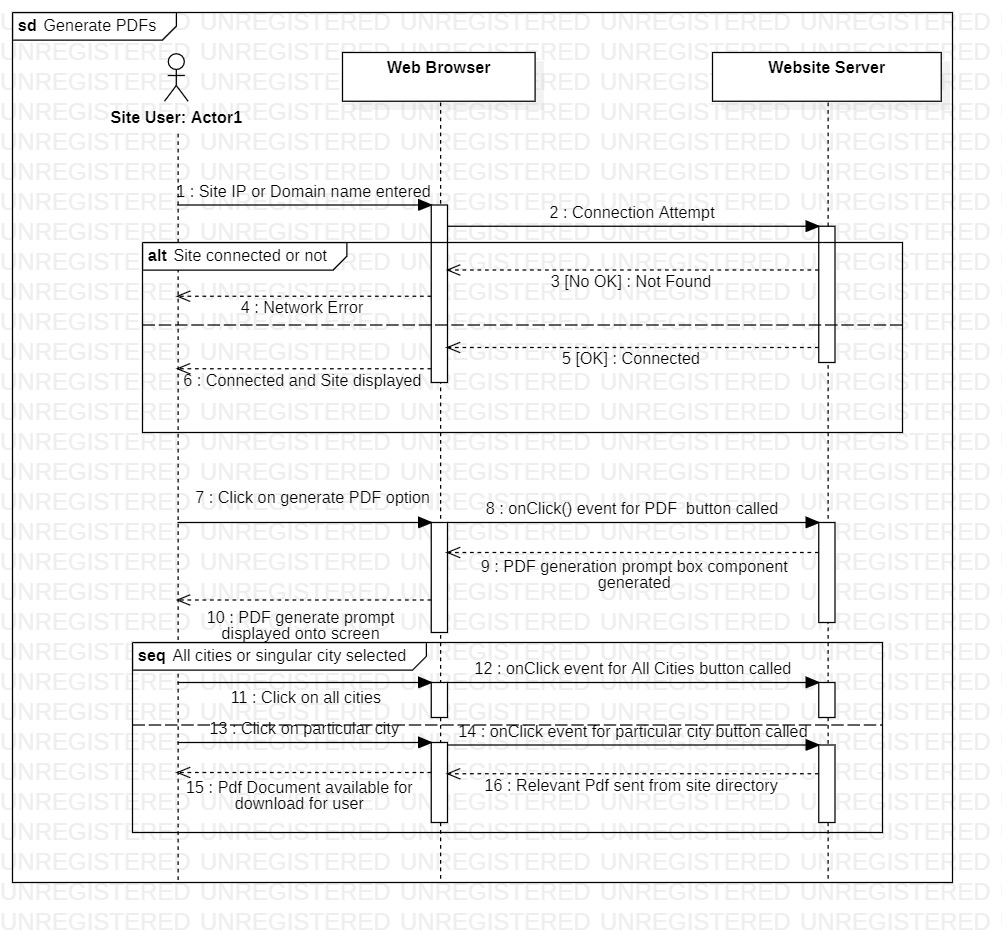
\includegraphics[width=\linewidth]{img/sequence-diagram-for-pdf.jpg}
  \caption{Sequence Diagram - Generate PDFs to Distribute Website}
\end{figure}

% Contact site maintainer
\begin{table}[H]
  \centering
  \refstepcounter{useCaseID}
  \resizebox{\linewidth}{!}{%
    \begin{tabular}{|p{.3\linewidth}|p{.7\linewidth}|}
      \hline
      \textbf{Use Case ID} & \theuseCaseID \\
      \hline
      \textbf{Use-Case Name} & Contact site maintainer \\
      \hline
      \textbf{Actors} & Victims or volunteers and Website maintainers \\
      \hline
      \textbf{Description} & Whenever a site user wants to contact with the maintainers, he or she can contact the maintainers to convey their opinions. \\
      \hline
      \textbf{Data} & Contact information \\
      \hline
      \textbf{Preconditions} & The contact information must be available. \\
      \hline
      \textbf{Stimulus} & User goes to about page and clicks the contact information. \\
      \hline
      \textbf{Basic Flow} & 
        \begin{minipage}[H]{\linewidth} 
          \begin{enumerate}[label=\textbf{Step \arabic*:},leftmargin=1.5\leftmargin]
            \item User clicks on ``\texttt{About Us / Contact}''
            \item User clicks on contact information link
            \item User is redirected to email app
          \end{enumerate}
        \end{minipage} \\
      \hline
      \textbf{Alternative Flow \#1} & - \\
      \hline
      \textbf{Alternative Flow \#2} & - \\
      \hline
      \textbf{Exception Flow} & - \\
      \hline
      \textbf{Post Conditions} & User starts browsing with the selected language in the \afetbilgi \\
      \hline
    \end{tabular}
  }
  \caption{Use Case - Contact site maintainer}
\end{table}

% Language Control
\begin{table}[H]
  \centering
  \refstepcounter{useCaseID}
  \resizebox{\linewidth}{!}{%
    \begin{tabular}{|p{.3\linewidth}|p{.7\linewidth}|}
      \hline
      \textbf{Use Case ID} & \theuseCaseID \\
      \hline
      \textbf{Use-Case Name} & Language control \\
      \hline
      \textbf{Actors} & Victims or Volunteer \\
      \hline
      \textbf{Description} & Whenever a site user wants to change the language of the website, he or she can change the language to acquire necessary information in another language. \\
      \hline
      \textbf{Data} & The translated website data \\
      \hline
      \textbf{Preconditions} & The data must be translated into the selected language. \\
      \hline
      \textbf{Stimulus} & User opens and changes the language of website on the language selector dropdown menu located on the right top corner of the website. \\
      \hline
      \textbf{Basic Flow} & 
        \begin{minipage}[H]{\linewidth} 
          \begin{enumerate}[label=\textbf{Step \arabic*:},leftmargin=1.5\leftmargin]
            \item User clicks and opens the dropdown language menu
            \item User selects the language that he or she wants to use
            \item The website and its data is updated according the selected language
            \item User starts browsing with the selected language
          \end{enumerate}
        \end{minipage} \\
      \hline
      \textbf{Alternative Flow \#1} & - \\
      \hline
      \textbf{Alternative Flow \#2} & - \\
      \hline
      \textbf{Exception Flow} & - \\
      \hline
      \textbf{Post Conditions} & User starts browsing with the selected language in the \afetbilgi \\
      \hline
    \end{tabular}
  }
  \caption{Use Case - Language control}
\end{table}

\vspace*{\fill}
\newpage

\subsection{Usability Requirements}

% Checked in grammarly
\begin{itemize}
    \item Being a website, users shall be able to easily navigate fast to sections concerning their relevant interest via clearly labeled explicitly placed buttons on the page.
    \item Users shall be able to understand the hierarchical/efficiently categorized portions of this website in the form of help categories and city selection.
    \item The website has been made easy to follow in multiple languages and has a simple plain design with center-placed buttons and efficient answering tables of information.
    \item Site maintainers have made the contents of this website accessible to the public, governmental organizations, media outlets, and sponsors/volunteers alike, in addition to its target of earthquake victims.
    \item The website has been optimized to work correctly on mobile devices and ensure access from anywhere.
    \item The website has contact details and socials of its managing community's details for fast feedback regarding complaints, and reviews from its users.
    \item Users must be able to gain fast access to pdf generation for distribution given stressful, emergency conditions in earthquake-stricken areas.
    \item Site maintainers must have verified as much information on details as possible for users to access while safeguarding their monetary and physical interests.
    \item Users shall be able to access the website at all times for secure third-party links. Hence the site maintainer's agenda is to host on widely-acclaimed services like Cloudflare.
    \item Maps should be able to serve not just geo-locations but also internal details, such as contact details involving physical addresses and phone numbers on description boxes for easy accessibility by victims and helper volunteers alike.
\end{itemize}

\subsection{Performance Requirements}

% Checked in grammarly
\begin{itemize}
    \item \textbf{High Availability:} To guarantee that it is always accessible, particularly in times of emergency when people require information and support, the \afetbilgi website should have high availability.
    \item \textbf{Fast Loading:} The website must load rapidly for users to access the required data immediately, especially in locations with sluggish internet connectivity. The site's various DNS(s)' health is regularly checked with CI/CD workflows.
    \item \textbf{Backup site data:} Via the backend of the GitHub workflow, the website is backed up and updated every 30 minutes with the latest version visible on any viewed webpage(from the site's hierarchy).
    \item \textbf{Adaptability:} The website has an adaptable design with straightforward, strategically positioned buttons suitable for desktops, laptops, tablets, and mobile devices.
    \item \textbf{Scalability:} The backend of the Cloudflare website should be able to handle high traffic, especially in times of emergency when it may increase dramatically.User-Friendly Interface: The website should have a simple, user-friendly interface that makes it simple for visitors to access available resources and obtain the information they need.
    \item \textbf{Multilingual Support:} To allow users who do not speak their native language to access the website's resources and information, the site maintainers have built it such that the website should support multiple languages.
    \item \textbf{Social media integration:} To encourage communication and information sharing among the impacted communities and other stakeholders, the website has been integrated with social media platforms like Discord and Twitter.
    \item \textbf{Accessibility:} \afetbilgi was created with accessibility in mind to make sure that persons with impairments can access the data and tools offered on the website, like different map views.
    \item \textbf{Information that is accurate and current:} \afetbilgi makes every attempt to offer accurate and current information regarding the earthquake, its effects, and the ongoing relief efforts.
    \item \textbf{Security and privacy:} To safeguard user personal information and guarantee that their donations and contributions are secure and free from frauds or thefts, third-party, external links with security and privacy in mind are chosen on the \afetbilgi website.
\end{itemize}

\subsection{Logical Database Requirements}

\afetbilgi does not currently have any relational database. To acquire the required data for both site and maps, it gets a JSON file from AWS and the code of website parses this JSON file according the path and the chosen option. For this purpose, it uses axios to send \texttt{GET} request to the \href{https://cdn.afetbilgi.com/latest.json}{\texttt{cdn.afetbilgi.com/latest.json}}. This request returns the \texttt{latest.json} file, which includes all the data required in the website. Although it may have drawback such as long load time, it may have advantages such as not loading any data after initial load.

To parse and upload the JSON file into the AWS, Github Workflows are used. Github Workflows parse and upload the \texttt{latest.json} by using the data, which collectors and validators collect and validate, periodically.

The relations between objects in the JSON file is shown at Figure \addnumbertofigure{1}. The code use these relations to parse the JSON correctly and show the included information in the JSON. If the system is updated to a relational database, the database can use the relations at the Figure \addnumbertofigure{1}.

\begin{figure}[H]
    \centering
    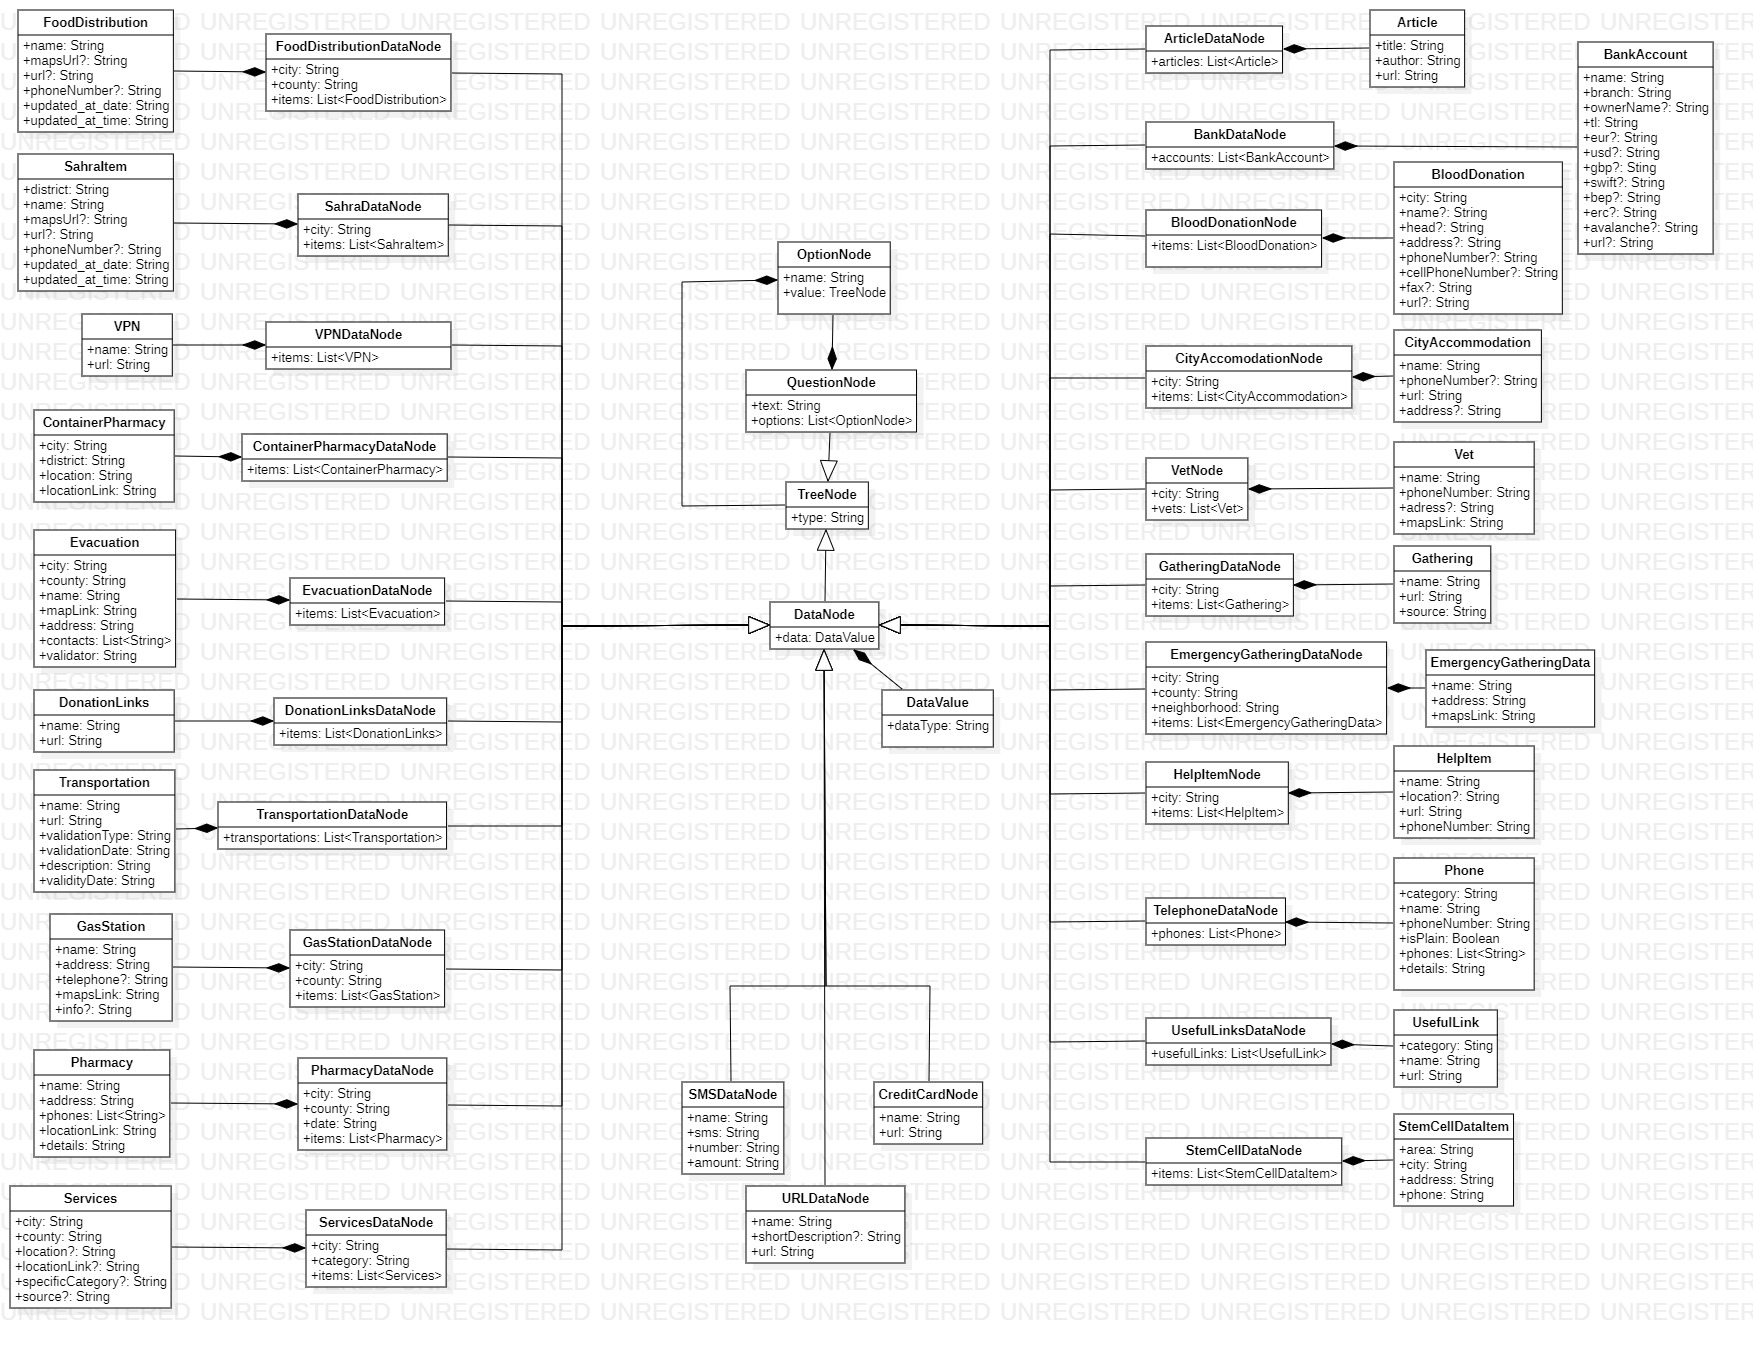
\includegraphics[width=\linewidth]{img/database.jpg}
    \caption{\texttt{latest.json} Object Structure}
\end{figure}

\subsection{Design Constraints}

% Checked in grammarly
The \afetbilgi website uses minimalistic design on its frontend site with central-placed, bold text clear buttons to allow users under potentially distressing conditions to scout and navigate through. Not only that, but due to a lack of proper open license given how the website was created for urgent use by students, the website still employs a proper backend system, at least, with Cloudflare to handle proxy DNS issues, GitHub CI/CD workflows to continuous update the website and check the various DNS(s) health, along with AWS to hold backup versions in cloud bucket instances too.

\vfill
\newpage

\subsection{System Attributes}

% Checked in grammarly
\begin{itemize}
  \item \textbf{Reliability:}
    \begin{itemize}[label=$\blacksquare$]
      \item All of the software involved in creating this website is open source to allow for inspection and improvement in future similar case scenarios.
      \item The website's DNS must always be in public health, along with the most recent updated information from the backend.
      \item GitHub CI/CD workflows must be regularly run to maintain website health with appropriate alerts in case of attacks/unusually high user traffic.
      \item Newly added pages must be checked with workflows to correspond to established data node interface conventions.
    \end{itemize}
  
  \item \textbf{Availability:}
    \begin{itemize}[label=$\blacksquare$]
      \item Site data must be backed up regularly to AWS for retrieval and archiving of past data before any potential updates.
      \item All of the sites involved DNS/domain names' health in being readily checked via HTTP request status with workflows to make sure they are active.
    \end{itemize}
  
  \item \textbf{Security:}
    \begin{itemize}[label=$\blacksquare$]
      \item Cloudflare is to be employed to safeguard against any potential high-traffic attacks.
      \item External sites mentioned and third-party links shall be evaluated by human personnel in the form of site contributors. Their validities/authenticities are judged accordingly to be placed and referred to on the website.
    \end{itemize}
    
  \item \textbf{Maintainability:}
    \begin{itemize}[label=$\blacksquare$]
      \item The site is regularly updated every 30 minutes as per CI/CD workflows from the latest open-source code repository.
    \end{itemize}
  
  \vfill
  \newpage
  
  \item \textbf{Portability:}
    \begin{itemize}[label=$\blacksquare$]
      \item \afetbilgi is made accessible with similar characteristics, such as having the same ease of use and clarity on mobile phones as on personal laptops/computers.
      \item PDF generation should be provided if the website details must be physically distributed to people.
    \end{itemize}
\end{itemize}

\subsection{Supporting Information}

% Checked in grammarly
It must be kept in mind that this website is an open-source efforted whose short-term immediate target period of use started just after the 6th of February and continues these days in the Spring of 2023 with proper maintenance. 

However, in the long term, this website might eventually be dissolved when monetary support for its backend services, domain registration, and so on ceases.
